\documentclass[__main__.tex]{subfiles}

\begin{document}

\qtitle{К}{18}
Рассмотрите задачу о движении электрона в одномерном потенциале, представляющем собой ступеньку высоты $U$ бесконечной ширины для случая, когда энергия электрона (а) $\varepsilon>U$, (б) $\varepsilon<U$. Прокомментируйте результаты.\\ 
\begin{gather*}
U(x) = 
\begin{cases}
	0, & x < 0\\
	U_0 & x > 0
\end{cases}
\end{gather*}
$a) \varepsilon > U_0$\\
Область $I(x < 0)$:\hspace{0.5cm} $\frac{\hbar^2}{2m}\frac{d^2\psi}{dx^2}+\varepsilon\psi = 0 \implies \frac{d^2\psi}{dx^2} + k_1^2\psi = 0; \hspace{0.5cm} k_1 = \frac{\sqrt{2m\varepsilon}}{\hbar}$
\begin{gather*}
	\psi_I = A_1e^{ik_1x} + B_1e^{-ik_1x}
\end{gather*}

Область $II(x > 0): \hspace{0.5cm} \frac{\hbar^2}{2m}\frac{d^2\psi}{dx^2} + (\varepsilon - U_0)\psi = 0 \implies \frac{d^2\psi}{dx^2}+k_2^2\psi=0; \hspace{0.5cm} k_2=\frac{\sqrt{2m(\varepsilon - U_0)}}{\hbar}$
\begin{gather*}
\psi_{II} = A_2e^{ik_2x}+B_2e^{-ik_2x}
\end{gather*}
Из непрерывности $\psi(x) и \frac{d\psi(x)}{dx}$ на границе $x=0$ 
\begin{gather}
\begin{cases}
\psi_I(0) = \psi_{II}(0)\\
\psi'_I(0) = \psi'_{II}(0)
\end{cases}
\begin{cases}
A_1 + B_1 = A_2\\
ik_1(A_1 - B_1) = ik_2A_2\\
\end{cases}
\begin{cases}
\llabel{k-18-b1}
B_1 = \frac{k_1 - k_2}{k_1 + k_2}A_1\\
A_2 = \frac{2k_1}{k_1 + k_2}A_1
\end{cases}
\end{gather}
\begin{wrapfigure}{L}{.3\linewidth}
	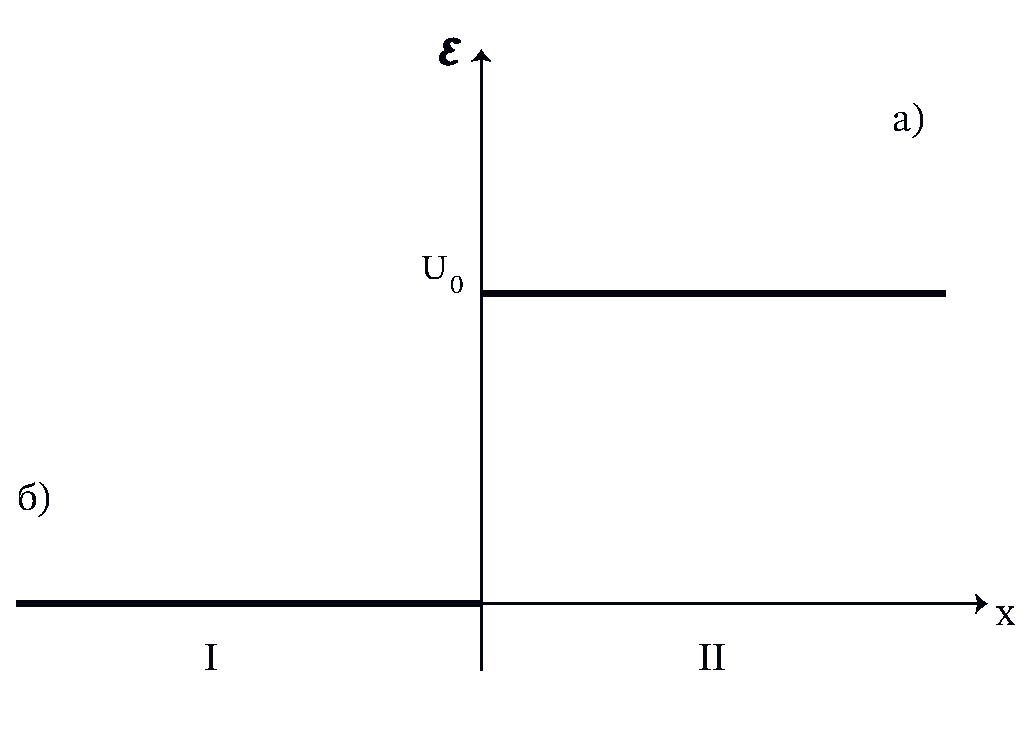
\includegraphics[scale=0.5]{k-18}
	\caption{}
	\llabel{k-18}
\end{wrapfigure}
Так как $\psi$ стационарное состояние, то
для стационарных состояний:
\begin{gather}
\nabla\vec{j} = 0
\llabel{k-18-j}
\end{gather}
\begin{gather*}
\vec{j} = Re[\psi^*\frac{\hbar}{im}\nabla\psi]
\end{gather*}
Величина вектора плотности тока вероятности в области I есть:
$$
j_1 = Re(A_1^*e^{-ik_1x} + B_1e^{-ik_1x})\frac{\hbar}{im}ik_1(A_1e^{ik_1x} - B_1e^{-ik_1x}) =\frac{\hbar k_1}{m}(|A_1|^2 - |B_1|^2)
$$
Величина вектора плотности тока вероятности в области II есть:
\begin{gather*}
j_2 = Re[A*_2e^{-ik_2x}\frac{\hbar}{im}ik_2A_2e^{ik_2x}] = \frac{\hbar k_2}{m}|A_2|^2\\
\lref{k-18-j} \implies j_1 = j_2 \implies k_1*(|A_1|^2 - |B_1|^2) = k_2|A_2|^2 | : k_1|A_1|^2\\
\frac{|B_1|^2}{|A_1|^2} + \frac{k_2|A_2|^2}{k_1|A_1|^2} = 1\\
R \equiv \frac{|B_1|^2}{|A_1|^2} \hspace{0.5cm} D \equiv \frac{k_2|A_2|^2}{k_1|A_1|^2}\\
\end{gather*}
$R$ - коэффициент отражения, $D$ - коэффициент прохождения\\
б) $\varepsilon < U_0$ \\
Область I $(X<0):$ всё так же, как и в случае (а): $\psi_I = A_1e^{ik_1x} + B_1e^{-ik_1x}$\\
Область II $(x>0): \frac{\hbar^2}{2m}\frac{d^2\psi}{2m}\frac{d^2\psi}{dx^2} + (\varepsilon - U_0)\psi = 0 \implies \frac{d^2\psi}{dx^2} - \kappa^2\psi = 0, \hspace{0.3cm} \kappa = \frac{\sqrt{2m(U_0-\varepsilon)}}{\hbar}\\\\
\psi_{II} = A_2e^{\mathcal{\kappa} x} + B_2e^{-\mathcal{\kappa x}}$ \\
Обнуляем $A_2$, так как первое слагаемое даёт $\infty$ на $\infty$\\
Граничные условия:
\begin{gather*}
\begin{cases}
\psi_I(0) = \psi_{II}(0)\\
\psi'_{I}(0) = \psi'_{II}(0)
\end{cases}
\begin{cases}
A_1 + B_1 = B_2\\
ik_1(A_1 - B_1) = -\mathcal{\kappa}B_2\\
\end{cases}
B_1 = -\frac{\mathcal{\kappa} + ik_1}{\mathcal{\kappa} - ik_1}A_1 \hspace{0.3cm} R = \frac{\mathcal{\kappa}^2 + k_1^2}{\mathcal{\kappa}^2 + k_1^2} = 1\\
\psi_I(x) = A_1(e^{ik_1x} - \frac{\mathcal{\kappa} + ik_1}{\mathcal{\kappa} - ik_1}e^{-ik_1x})\\
\psi_{II}(x) = \frac{-2ik_1}{\mathcal{\kappa} - ik_1}A_1e^{-\mathcal{\kappa}x}\\
|\psi_{II}|^2 = \frac{4k_1^2}{\mathcal{\kappa}^2 + k_1^2}|A_1|^2e^{-2\mathcal{\kappa}x}
\end{gather*}
\end{document}